\documentclass[12pt,fleqn]{article}
\setlength{\parindent}{0pt}
\usepackage{graphicx}
\usepackage{cancel}
\usepackage{listings}
\usepackage[latin5]{inputenc}
\usepackage{color}
\setlength{\parskip}{8pt}
\setlength{\parsep}{0pt}
\setlength{\headsep}{0pt}
\setlength{\topskip}{0pt}
\setlength{\topmargin}{0pt}
\setlength{\topsep}{0pt}
\setlength{\partopsep}{0pt}
\setlength{\mathindent}{0cm}

\begin{document}
Ders 16

Konumuz cift entegraller (double integrals). Bildigimiz gibi su sekilde bir
entegral aldiginizda

\[ \int_a^bf(x)dx = \textit{f'in [a,b] arasindaki bolumdeki alani} \]

anlamina gelir. 

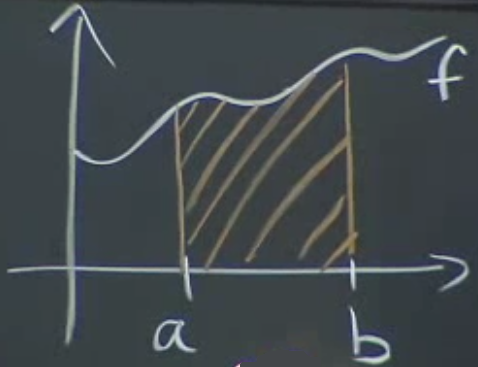
\includegraphics[height=2cm]{16_1.png}

Eger $f$ negatif ise o zaman alan eksen altinda yer alacaktir. 

Iki degiskenli fonksiyonlar icin benzer bir sey yapilabilir, 3 boyutlu
uzayda $z=f(x,y)$ fonksiyonumuzu grafikledigimizi dusunelim, bu bir yuzey olusturur,
yuzeyin altinda kalan ``hacim'' hesaplanabilir, ki bu hesap cift
entegraller ile mumkun olmaktadir. 

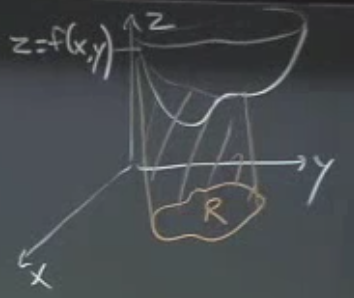
\includegraphics[height=3cm]{16_2.png}

Cift entegral icin $f(x,y)$'miza bakiyoruz, sonra ``uzerinden entegrasyon
isleminin yapilacagi'' bolge $R$'i seciyoruz. Tek entegraldeki $[a,b]$
araligi gibi, ama bu sefer bolge bir cizgi degil, bir alan. Entegral soyle
gosteriliyor 

\[ \int \int_R f(x,y) dA \]

Formulde $dA$'nin anlami ``$A$ alaninin bir parcasi'' demek. Hesaplama
vakti gelince bu notasyonun daha somut halini gorecegiz. 

Biraz daha matematiksel / teorik / detayli (rigorous) olarak bakmak
gerekirse; tek entegralde $[a,b]$ araligini ufak parcalara bolup, o
bolumlerin genisligini $f$ ile carptigimizi ve sonuclari birbirine
topladigimizi hayal ediyorduk. 

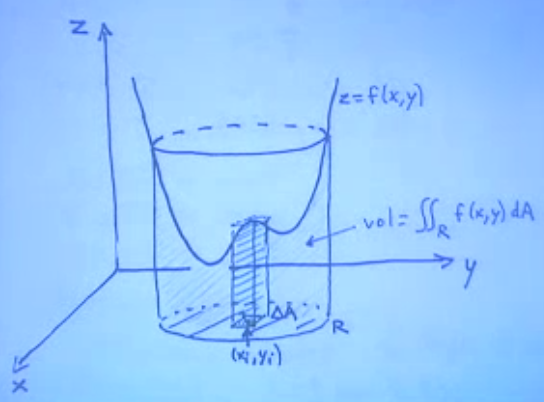
\includegraphics[height=4cm]{16_3.png}

Cift entegralde bu ufak kesit bir kenari $\Delta x$ diger kenari $\Delta y$ olan
bir dikdortgen alani $\Delta A$. Sonra $\Delta A$'yi o noktadaki $f$ ile
carpiyoruz, ve resimde cizgili gosterilen hacmi buluyoruz. Tum entegral icin
bu hacimleri topluyoruz. Entegral matematiksel olarak bir limit olarak
gosteriliyor, yani $\Delta A$ gitgide ufaliyor. 

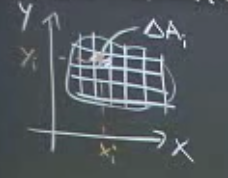
\includegraphics[height=3cm]{16_4.png}

Toplam soyle gosterilebilir

\[ \sum_i f(x_i,y_i) \ \Delta A_i \]

ve $\Delta A \to 0$ uzerinden limit aliyoruz, cift entegrali elde ediyoruz. 

Tabii ki entegral hesabini yaparken, tek ya da cift olsun, her seferinde
ufak parcalara bolup, toplam ile ugrasmiyoruz. Entegral kavraminin bize
sagladigi formulsel kolayliklari kullaniyoruz.

Formulsel olarak cift entegral hesabi yapmak icin ``tarayici bir
duzlem'' hayal edebiliriz. Mesela alttaki resimde $yz$ duzlemine paralel
duzlemin arkadan one dogru onune gecerek her seyi taradigini dusunelim, her
duzlem $x=x_0$'a tekabul ediyor, o zaman tarama sirasinda farkli $x_0$'lar
kullaniyoruz.

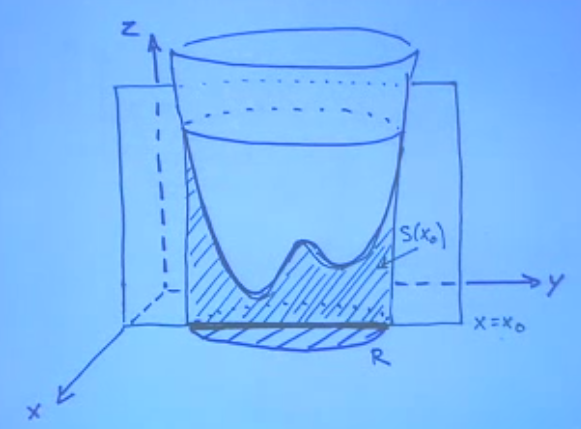
\includegraphics[height=4cm]{16_5.png}

Tek bir $x_0$ ``fotografina'' bakarsak, o duzlemin uzerinde dusen $f$
yansimasinin altindaki alanin normal (tek) bir entegral olarak
hesaplanabilecegini gorebiliriz. One dogru her hareket bir $\Delta x$ ise,
oradan her ufak hareketin hacmini buluruz. Tum bu ufak hacimleri toplarsak,
toplam hacmi elde ederiz. Fotograftaki her alana $S(x)$ adi verelim.

Yani 

\[ Hacim = \int S(x) dx \]

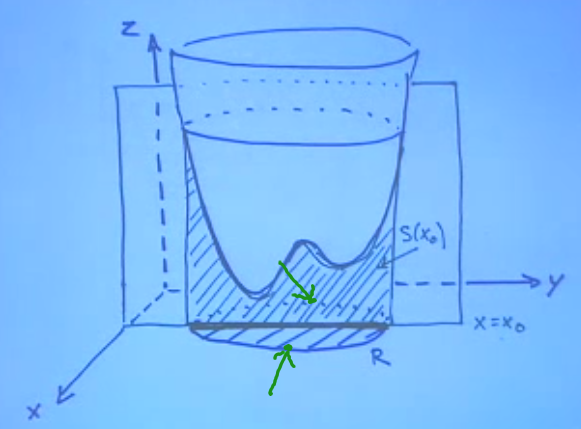
\includegraphics[height=3cm]{16_6.png}

Taramanin sinirlari ise ustteki yesil oklarla gosteriliyor, degerleri
$x_{min}$, $x_{maks}$ olarak gosteribiliriz, yani

\[ Hacim = \int_{x_{min}}^{x_{max}} S(x) dx \]

$S(x)$'in kendisi de bir entegraldir, fakat $y$ degiskeni uzerinden, cunku
fotograf sirasinda $x$ sabit. 

\[ S(x) = \int f(x,y) dy \]

$y$'nin alt ust limitleri $x=x_0$ olmak uzere (cunku o kesit uzerindeyiz)
$R$'nin baslangic ve bitis degeridir. Yani

\[ S(x) = \int_{y_{min}(x)}^{y_{max}(x)} f(x,y) dy \]

Bu onemli bir nokta: $y$'nin limit degerleri belli bir $x$ degerine
bagli. Alttaki resimde bu daha iyi anlasilabilir. 

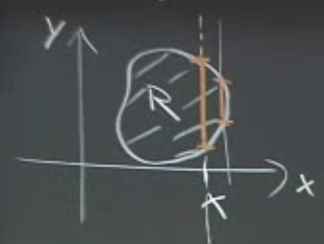
\includegraphics[height=3cm]{16_7.png}

Ustteki resim onceki 3 boyutlu resmin bir kusbakisi. Her kesit bir cizgi
olarak gozukuyor, eger buyuk kirmizi cizgi (kesit) uzerinde isek, baslangic
bitis $y$ degerleri ile hesaplanan alan entegrali, kucuk kirmizi cizgi
(kesite) uzerindekine nazaran degisik olacaktir.

\[ A = \int_{x_{min}}^{x_{max}} 
\bigg[ 
\int_{y_{min}(x)}^{y_{max}(x)} f(x,y) dy 
\bigg] dx
 \]


Bu isleme tekrarli entegral (iterated integral) ismi de veriliyor, cunku
bir anlamda fonksiyonun uzerinden iki kere gecmemiz gerekiyor. 

Onemli bir nokta oldugu icin tekrar vurgulayayim: Dis entegraldaki
$x_{min}, x_{max}$ degerleri birer sayi sadece. Ic entegraldaki
$y_{max}(x)$ degerleri ise dis entegraldaki $x$'e bagli. 

Ornek

\[ z = 1 - x^2 - y^2 \]

\[ 0 \le x \le 1 \]

\[ 0 \le y \le 1 \]

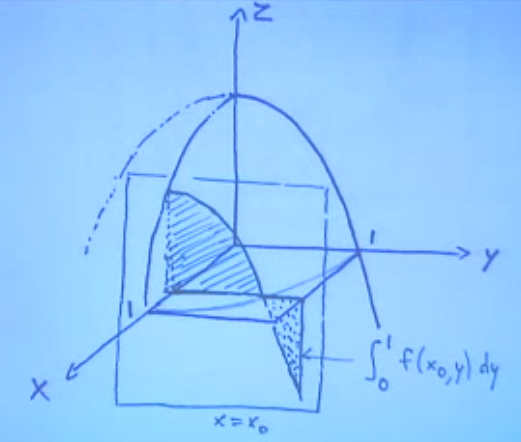
\includegraphics[height=5cm]{16_8.png}

\[ \int_0^1 \int_0^1  1-x^2-y^2 \ dy \ dx \]

Ilk once ic entegrali hesaplayacagim, $x$ sabit kalacak. 

1) Ic Entegral

\[ \int_0^1 (1-x^2-y^2) dy = [y - x^2y - \frac{y^3}{3}]_0^1 \]

\[ = (1 - x^2 - \frac{1}{3}) - 0 = \frac{2}{3} - x^2\]

Son formul sadece $x$'in fonksiyonu, bu noktada artik $y$ kalmadi, cunku
$y$ entegrasyon degiskenimizdi. Ama hala $x$ var, cunku kesit uzerindeki
alan $x$'in degerine bagli. 

2) Dis Entegral 

\[ \int_0^1 (\frac{2}{3} - x^2)dx = [\frac{2}{3}x - \frac{1}{3}x^3]_0^1 = 
\frac{1}{3}
 \]

Sonucu bulduk. 

Ilk basta $dA$ notasyonunu kullanmistik, $dA$ nereye kayboldu? $dA$ ufak
kesit dikdortgen alan degil miydi? Hesabi yaparken $dy \ dx$ kullandik,
$dy,dx$ dikdortgenin kenarlari gibi gorulebilir, dikdortgen alani
kenarlarinin carpimina esittir, o zaman 

\[ dA = dy \ dx \]

Peki niye $dx \ dy$ kullanmadik? Sira istenilen sekilde secilebilir, hangi
entegrali daha once hesaplamak istedigimize gore once $y$, sonra $x$, ya da
tam tersi kullanabiliriz. Bu secim dikkatli yapilmali, cunku degisken
onceligi sinir degerlerini direk etkileyecek. 

Tabii teorik olarak oncelik farketmiyor, fakat pratikte bazen bir degiskene
gore entegrasyon digerine gore cok zor olabiliyor, o zaman otekinin
entegrasyonu one aliniyor, vs.

Ornek

Ustteki ornekteki ayni fonksiyon, ama degisik bir bolge kullanalim. 

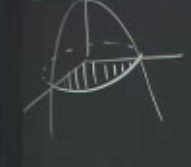
\includegraphics[height=3cm]{16_9.png}

Yeni bolge ceyrek disk (quarter disk) olsun. $xy$ uzerindeki yansimasi
soyle. 

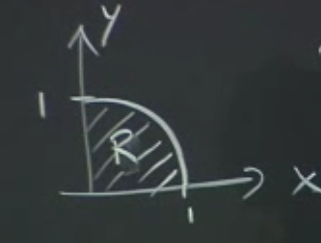
\includegraphics[height=3cm]{16_10.png}

\[ R = \textit{ceyrek disk}  \]

\[ x^2 + y^2 \le 1 \]

\[ x \ge 0, y \ge 0 \]

Ayni entegral ama degisik sinir degerleri, cunku ilk ornegin 3d resmine
bakarsak, $xy$ duzleminde bir ceyrek cember var, o cember icindeki bolgede
alan pozitif, disinda alan negatif. 













\end{document}
